\documentclass[a4paper, czech]{article}

\usepackage[czech]{babel}
\usepackage{indentfirst}
\usepackage{graphicx}
\usepackage{float}
\usepackage[margin=1.5cm]{geometry}
\usepackage{booktabs}
\usepackage{amsmath}
\usepackage{xcolor}
\usepackage{multirow}
\usepackage{tabularray}
\usepackage{bold-extra}
\usepackage{circuitikz}
\usepackage{caption}
\usepackage{subcaption}


\begin{document}
\begin{table}[H]
    \centering
    \begin{tblr}{
        cell{1}{1} = {c = 2, r = 4}{c}, % Logo
        cell{1}{4} = {c = 3}{c}, % Předmět
        cell{2}{4} = {c = 3}{c}, % Jméno
        cell{3}{4} = {}{c}, % Ročník
        cell{3}{6} = {}{c}, % Studijní skupina
        cell{4}{4} = {}{c}, % Spolupracoval
        cell{4}{6} = {}{c}, % Mereno dne
        cell{5}{1} = {c = 2}{55mm}, % Kontroloval
        cell{5}{3} = {c = 2}{55mm}, % Hodnoceni
        cell{5}{5} = {c = 2}{55mm}, % Dne
        cell{6}{2} = {c = 5}{}, % Nazev ulohy
        cell{7}{1} = {}{c}, % Číslo úlohy
        cell{7}{2} = {c = 5}{c}, % Název úlohy
        vline{1,2,7} = {1.2pt},
        vline{3,5},
        hline{1,5,6,8} = {1.2pt},
        hline{2,3,4}
        }
        
\includegraphics{logo_fekt.png} & & \textsuperscript{Předmět} & \large \textbf{Měření v audiotechnice} \\
             & & \textsuperscript{Jméno} & \large \textbf{Karolína Šebestová} \\
             & & \textsuperscript{Ročník} & \large \textbf{3.} & \textsuperscript{Studijní skupina} & \large \textbf{St 14:00} \\
             & & \textsuperscript{Spolupracoval} & \large \textbf{Filip Kokavec} & \textsuperscript{Měřeno dne} & \large \textbf{6.11.2024} \\
        \textsuperscript{Kontroloval} & & \textsuperscript{Hodnocení} & & \textsuperscript{Dne} \\
        \textsuperscript{Číslo úlohy} & \textsuperscript{Název úlohy} \\
        \Large \textbf{6B} & \Large \textsc{\textbf{Princip A/Č převodníku s dvojitou integrací}} \\
    \end{tblr}
\end{table}

\section{Zadání}

\begin{itemize}
    \item Obeznamte se s principem předloženého převodníku s dvojitou integrací. Proměřte jeho převodní charakteristiku, zakreslete napětí na výstupu integrátoru, ověřte jeho potlačení střídavého rušivého signálu.
    \item Graficky znázorněte naměřené převodní charakteristiky převodníku s dvojitou integrací.
\end{itemize}

\section{Teoretický úvod}

Ve všech číslicových měřících přístrojích je použit A/Č převodník, který převádí vstupní spojitý signál na časově diskrétní číselnou hodnotu, která je zobrazena na displeji zařízení.
Hodnota se převádí použitím kvantizace (diskretizace v čase).

V měřících přístrojích se nejčastěji střetáváme s převodníky s dvojitou integrací, který má výhodu spočívající v potlačení rušení z elektrické sítě.
Je používán jak ve voltmetrech t ak i v multimetrech.
Jeho elektrické vlastnosti dokáží také eliminovat časové nestability obvodových prvků R a C a také kmitočtu oscilátoru.

V přípravku v této úloze je použit integrovaný obvod ICL7135, který je řízen hodinovým signálem z laboratorního generátoru.
Bez tohoto hodinového signálu není schopen funkce.

\begin{figure}[H]
    \centering
    \begin{circuitikz}
        % Referenční napětí
        \draw (0,0) node[draw, rectangle, line width=1, align=center, minimum height=1cm, inner xsep=7.5](refNap){Referenční\\napětí}
        % Dělič
        (refNap.east) to node[pos=0.5, circ](uzel1){} ++(0.5,0) node[draw, rectangle, line width=1, align=center, anchor=west, minimum height=1cm, inner xsep=7.5](delic){Dělič}
        % Sumátor
        (delic.east) to node[pos=0.25, circ](uzel2){} ++(2.5,0) ++(0,-0.25) node[draw, rectangle, line width=1, align=center, anchor=west, minimum height=1cm, inner xsep=7.5](sumator){Sumátor}
        % ICL7135
        (sumator.east) to node[pos=0.6, label={[label distance=-5]below:$U_X$}]{} ++(2,0) ++(0,0.25) node[draw, rectangle, line width=1, align=center, anchor=west, minimum height=2cm, inner xsep=7.5](ICL){ICL7135} (ICL.west) ++(0,0.25) coordinate(ICLa)
        (uzel1) to ++(0,0.75) coordinate(X) to (X -| sumator.east) to ++(0.5,0) coordinate(X) to (X |- ICLa) to node[pos=0.5, label={[label distance=-5]above:$U_{ref}$}]{} (ICLa)
        % Číslicový voltmetr
        (uzel2) to node[pos=0.9, label={[label distance=-5]right:$U_X$}]{} ++(0,-2) node[draw, rectangle, anchor=north, align=center, inner xsep=7.5, line width=1](voltmetr){Číslicový\\voltmetr}
        % Displej
        (ICL.east) ++(0,0.6) to ++(1.5,0) node[draw, rectangle, anchor=west, line width=1, minimum height=1cm, inner xsep=7.5](displej){Displej}
        % Osciloskop
        (ICL.east) ++(0,-0.6) to node[pos=0.6, label={[label distance=-5]above:$U_{INT}$}]{} ++(1.5,0) node[draw, rectangle, anchor=west, line width=1, minimum height=1cm, inner xsep=7.5](osciloskop){Osciloskop}
        % Generátor
        (ICL.south) to node[pos=0.75, label={[label distance=-5]right:$f_{INT}$}]{} ++(0,-1) coordinate(X) to (X -| osciloskop.west) ++(0,-0.25)
        node[draw, rectangle, anchor=west, minimum height=1cm, line width=1, inner xsep=7.5](generator){Generátor}
        (sumator.west) ++(0,-0.25) to ++(-0.5,0) coordinate(X) to (X |- generator.west) to node[pos=0, label={[label distance=-5]right:$f_{ru \check{s}}$}]{} ++(0,-0.25) coordinate(X) to (X -| generator.west)
        ;
        % Obdélník s názvem
        \draw [line width=1.2] (-1.3,1.5) rectangle (11.35,-1.2) node[pos=0.5](X){}
        (X) ++(0,1) node[]{\textbf{Převodník s dvojitou integrací}};
    \end{circuitikz}
    \caption{Blokové schéma zapojení s přípravkem převodníku s dvojitou integrací}
\end{figure}

\section{Výsledky měření}

\subsection{Tabulky}

\begin{table}[H]
    \catcode`\-=12
    \centering
    \caption{Převodník s dvojitou integrací}
    \begin{tabular}{ll|ccccccccc}
        \toprule
        $U_X$  & [V]  & 0,1   & 0,2   & 0,3   & 0,4   & 0,5   & 0,6   & 0,7   & 0,8   & 0,9   \\
        \cmidrule(rl){1-11}
        $N$   & [-]  & 1000  & 2003  & 3005  & 4007  & 5008  & 6010  & 7012  & 8013  & 9015  \\
        $N_{ID}$ & [-]  & 1000  & 2000  & 3000  & 4000  & 5000  & 6000  & 7000  & 8000  & 9000  \\
        $\delta_N$  & [\%] & 0,000 & 0,150 & 0,167 & 0,175 & 0,160 & 0,167 & 0,171 & 0,163 & 0,167 \\
        \bottomrule
    \end{tabular}
\end{table}

\begin{table}[H]
    \catcode`\-=12
    \centering
    \caption{Převodník s dvojitou integrací}
    \begin{tabular}{cccc}
        \toprule
        $U_X$  & $T_1$  & $T_2$ & $N_{ID}$  \\
        \cmidrule(rl){1-1}
        \cmidrule(rl){2-2}
        \cmidrule(rl){3-3}
        \cmidrule(rl){4-4}
        V   & ms  & ms & -    \\
        \midrule
        0,3 & 100 & 30 & 3000 \\
        0,6 & 100 & 61 & 6100 \\
        0,9 & 100 & 91 & 9100 \\
        \bottomrule
    \end{tabular}
\end{table}

\subsection{Snímky obrazovky osciloskopu}

\begin{figure}[H]
    \centering
    \begin{subfigure}{0.49\textwidth}
        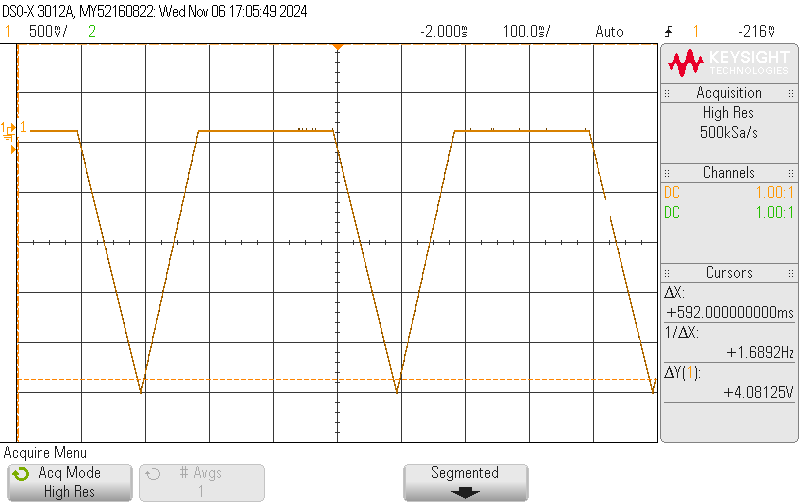
\includegraphics[width=\textwidth]{osc_6B_1.png}
        \caption{$U_X = 0,9\,$V}
    \end{subfigure}
    \hfil
    \begin{subfigure}{0.49\textwidth}
        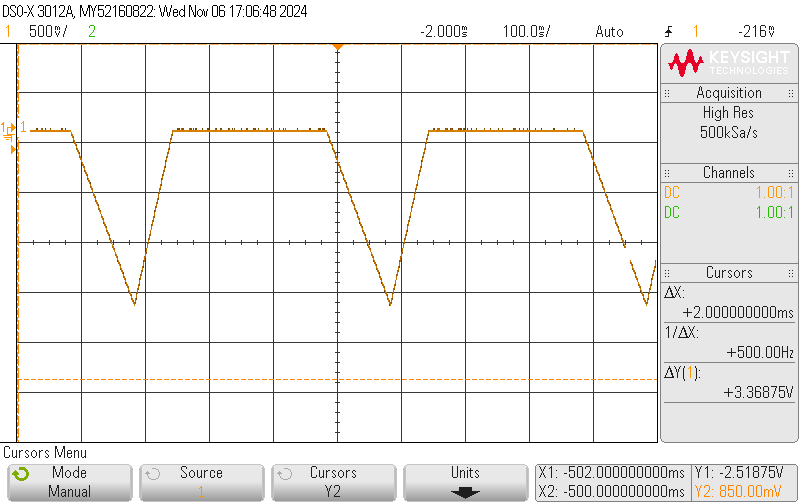
\includegraphics[width=\textwidth]{osc_6B_2.png}
        \caption{$U_X = 0,6\,$V}
    \end{subfigure}

    \begin{subfigure}{0.49\textwidth}
        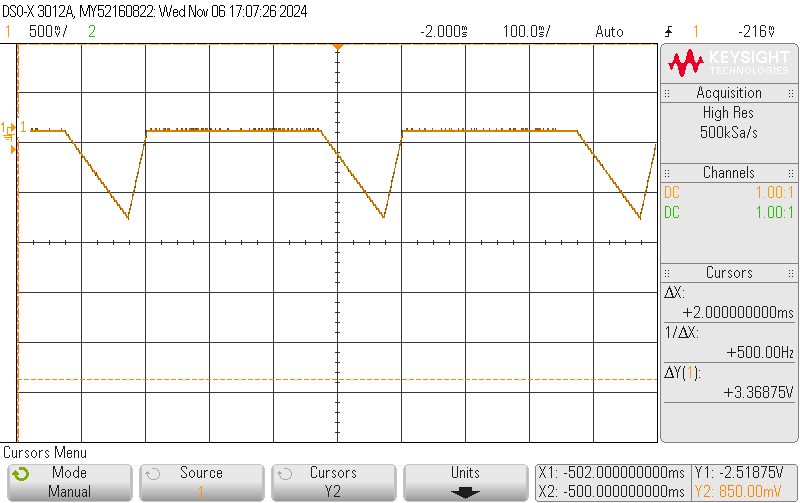
\includegraphics[width=\textwidth]{osc_6B_3.png}
        \caption{$U_X = 0,3\,$V}
    \end{subfigure}
    \caption{Průběhy výstupního napětí generátoru pro jednotlivá vstupní napětí $U_X$}
\end{figure}

\begin{figure}[H]
    \centering
    \begin{subfigure}{0.49\textwidth}
        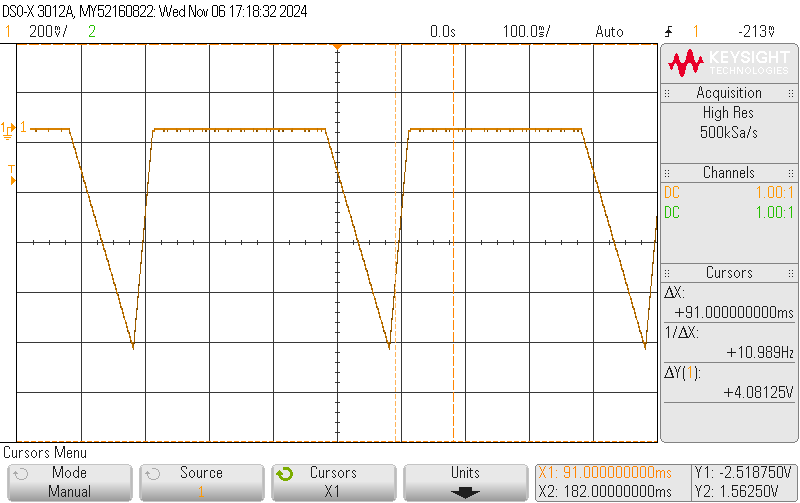
\includegraphics[width=\textwidth]{osc_6B_4.png}
        \caption{bez rušení}
    \end{subfigure}
    \hfil
    \begin{subfigure}{0.49\textwidth}
        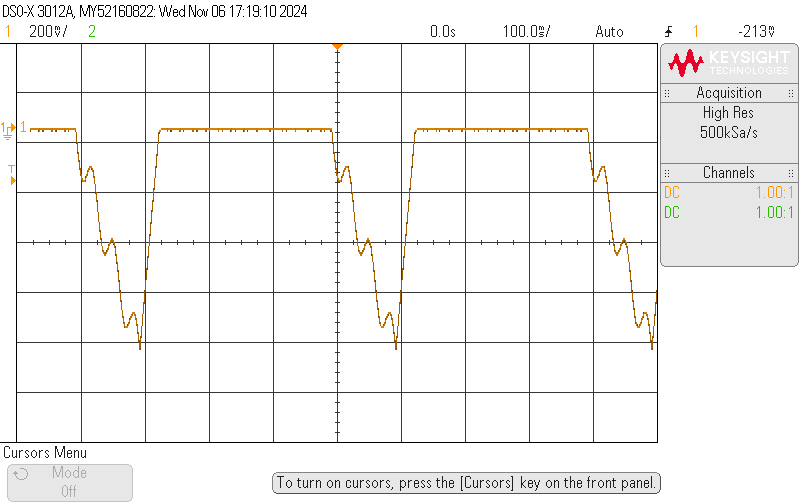
\includegraphics[width=\textwidth]{osc_6B_5.png}
        \caption{$f_{ru \check{s}} = 30\,$Hz}
    \end{subfigure}

    \begin{subfigure}{0.49\textwidth}
        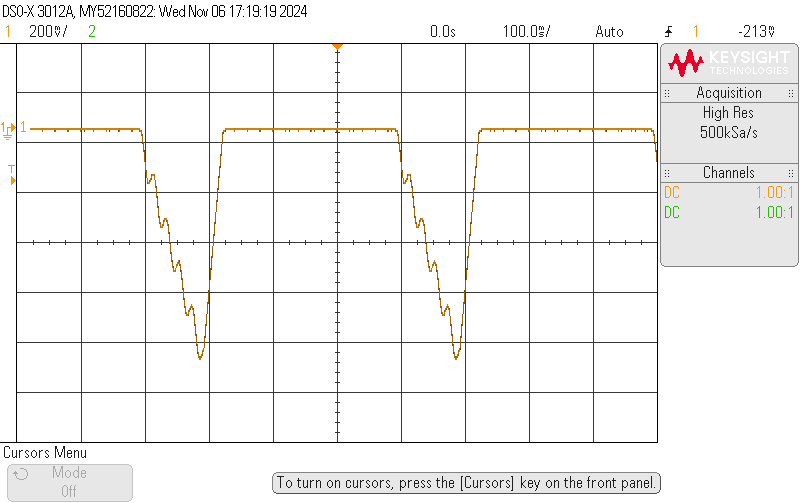
\includegraphics[width=\textwidth]{osc_6B_6.png}
        \caption{$f_{ru \check{s}} = 50\,$Hz}
    \end{subfigure}
    \caption{Vliv rušení na průběh výstupního napětí generátoru}
\end{figure}

\subsection{Příklady výpočtu}

\begin{enumerate}
    \item Ideální stav čítače po ukončení převodu
    \begin{multline*}
        N_{ID} = \textcolor{teal}{N_C \cdot \frac{U_X}{U_{ref}}} = 10\,000 \cdot \frac{0,2\,V}{1\,V} = \underline{\underline{2\,000}} \hfill
    \end{multline*}
    \item Relativní chyba naměřené hodnoty čítače převodníku
    \begin{multline*}
        \delta_N = \textcolor{teal}{\frac{N - N_{ID}}{N_{ID}} \cdot 100\,\%} = \frac{2\,003 - 2\,000}{2\,000} \cdot 100\,\% = \underline{\underline{0,15\,\%}} \hfill
    \end{multline*}
    \item Ideální stav čítače po ukončení převodu ze změřených časů $T_1$ a $T_2$
    \begin{multline*}
        N_{ID} = \textcolor{teal}{N_C \cdot \frac{T_2}{T_1}} = 10\,000 \cdot \frac{30\cdot10^{-3}\,s}{100\cdot10^{-3}\,s} = \underline{\underline{3\,000}} \hfill
    \end{multline*}
    \item Změna údaje displeje vlivem sériového rušení
    \begin{multline*}
        \Delta N =  4076 - 3000 = \underline{\underline{1076}} \hfill
    \end{multline*}
    \item Ideální potlačení sériového rušivého signálu
    \begin{multline*}
        SMR_{teor} = \textcolor{teal}{20 \cdot log \left(\frac{\pi \cdot T_1 \cdot f_{ru \check{s}}}{\left|sin\left(\pi \cdot T_1 \cdot f_{ru \check{s}}\right)\right|}\right)} = 20 \cdot log \left(\frac{\pi \cdot 100\cdot10^{-3}\,s \cdot 12,5\,Hz}{\left|sin\left(\pi \cdot 100\cdot10^{-3}\,s \cdot 12,5\,Hz\right)\right|}\right) = \underline{\underline{14,89\,dB}} \hfill
    \end{multline*}
    \item Naměřené potlačení sériového rušivého signálu
    \begin{multline*}
        SMR_{mer} = \textcolor{teal}{20 \cdot log \left(\cfrac{U_{ru \check{s}}}{\left|\Delta N\right| \cdot \cfrac{U_{ref}}{N_C}}\right)} = 20 \cdot log \left(\cfrac{0,5\,V}{\left|1\,076\right| \cdot \cfrac{1\,V}{10\,000}}\right) = \underline{\underline{13,34\,dB}} \hfill
    \end{multline*}
\end{enumerate}

\section{Seznam použitých přístrojů}

\begin{itemize}
    \item Číslicový osciloskop Agilent DSO-X 3014A, v.č. MY51290304
    \item Číslicový laboratorní multimetr Metra M1T390, v.č. 40004281793
    \item Číslicový laboratorní signálový generátor Siglent SDG 2042X, v.č. SDG2XCAC2R0604
\end{itemize}

\section{Závěr}

Cílem tohoto námi provedeného měření bylo určit převodní charakteristiku převodníku a taktéž ověřit jeho potlačení rušivého střídavého signálu.

Relativní chyby naměřených hodnot $\delta_N$ jsou relativně malé, nejvyšší znich je 0,175\,\% při $U_X = 0,4\,$V.
Tyto odchylky jsou nejpravděpodobněji způsobeny nedokonalostí v linearitě měřeného převodníku.

Při měření hodnoty čítače N na fázi dosáhl převodník nejvyššího rozdílu $\Delta N = 1076$.
Ideální potlačení sériového rušivého signálu bylo námi vypočteno na hodnotu 14,89\,dB.
Naměřené potlačení sériového rušivého signálu bylo určeno na hodnotu 13,36\,dB.

Maximální potlačení síťového rušivého napětí by mělo nastat, pokud dobu integrace $T_1$ nastavíme na hodnotu periody rušivého napětí 20 ms, nebo násobku této hodnoty. Časový Integrál bude při násobcích této hodnoty vždy nulový.

\end{document}